
\documentclass[12pt]{article}
\usepackage[margin=1in]{geometry}
\usepackage{amsmath, amssymb, amsthm, graphicx, hyperref}
\usepackage{enumerate}
\usepackage{fancyhdr}
\usepackage{multirow, multicol}
\usepackage{tikz}
\pagestyle{fancy}
\fancyhead[RO]{Eliot Brown Spring 2020}
\fancyhead[LO]{MA-UY 2314: Discrete Mathematics}
\usepackage{comment}
\newif\ifshow
\showfalse
\usepackage{centernot}


\begin{document}

\begin{center}
  \textbf{\Large Homework 5} \\
Due: Wednesday  March. 4 by 11:59pm
via Gradescope
\end{center}

\hrule

\vspace{0.25in}

\begin{enumerate}
\item (18 points) Section 14 problem 14.4.  \\
\textbf{Solution}
 A) Reflexive, Transitive, Symmetric \\
 B) Irreflexive, Anti Symmetric  \\ 
 C) Reflexive, Symmetric, Transitive  \\
 D) Reflexive, Symmetric  \\
 E) Irreflexive, Symmetric  \\
 F) Irreflexive, Anti Symmetric, Transitive  \\


\item (9 points)  14.6, 14.7(d), 14.7(e).  When doing problems 14.7(d) and (e), prove your answer.
\textbf{14.6 Solution} \\ 
A.) R = \{(x,y): \mid x - y \mid <= 2\} \\
B.) T \\
C.) F, if R = {(1,2),(2,3),(3,4)}, then 1\mathrel{R}2, 2\mathrel{R}3, 3\mathrel{R}4 \\
D.) F, if R = {(1,2),(2,3),(3,4)}, then 1\mathrel{R}2, 1 != 2 \\
E.)T \\
F.) F, if 1 \mathrel{R} 2, & 2\mathrel{R} 4, 1 \not\mathrel{R} 4 \\

14.7(d)$R=\{(x,y):x,y \in \mathbb{N},y|x \} $\\

Assume $A=\{(x,y):x,y \in \mathbb{N},y|x \} $\\
we must prove the following statements:
$(x,y) \in R^{-1} \rightarrow (x,y) \in A $\\
$(x,y) \in A \rightarrow (x,y) \in R^{-1} $\\

proof of \textbf{statement 1}:\\
Assume $(x,y) \in R^{-1}$\\
so, $(y,x) \in R$\\
so $y \mid x$\\
so $(x,y) \in A$\\

proof of \textbf{statement 2}:\\
Assume $(x,y) \in A$\\
so $y \mid x$\\
so $(y,x) \in R$\\
$(x,y) \in R^{-1} \;\; \square$\\


14.7(e)$R=\{(x,y):x,y \in \mathbb{Z},yx>0 \} $\\
Assume $A=\{(x,y):x,y \in \mathbb{N},yx>0 \} $\\
we must prove the following statements:
$(x,y) \in R^{-1} \rightarrow (x,y) \in A $\\
$(x,y) \in A \rightarrow (x,y) \in R^{-1} $\\

proof of \textbf{statement 1}:\\
Assume $(x,y) \in R^{-1}$\\
so $(y,x) \in R$\\
so $yx>0$\\
so $(x,y) \in A$\\

proof of \textbf{statement 2}:\\
Assume $(x,y) \in A$\\
so $yx>0$\\
so $(y,x) \in R$\\
so $(x,y) \in R^{-1} \;\; \square$\\

\item (3 points)  14.12.  Prove your result.  This will mimic the work you've done in problems 14.7(d) and (e).  \\

14.12 the answer will be $\geq$.\\
$R^{-1}=\{(x,y):x,y \in \mathbb{Z},y \leq x \}$\\

let the relation $A=\{(x,y):x,y \in \mathbb{Z},y \leq x \}$\\
we must prove the following statements:
$(x,y) \in R^{-1} \rightarrow (x,y) \in A $\\
$(x,y) \in A \rightarrow (x,y) \in R^{-1} $\\

proof of \textbf{statement 1}:\\
Assume $(x,y) \in R^{-1}$\\
so $(y,x) \in R$\\
so $y \leq x$\\
so $(x,y) \in A$\\

proof of \textbf{statement 2}:\\
Assume $(x,y) \in A$\\
so $y \leq x$\\
so $(y,x) \in R$\\
so $(x,y) \in R^{-1} \;\; \square$\\

\item (9 points)  14.13. 

 14.13(a) let $A=\{1,2\}, R= \{(1,1)\}$, this is false for both reflexive and irreflexive\\
 
 14.13(b) let $A= \emptyset, R = \emptyset$, this is both reflexive and irreflexive\\

\item (6 points) 14.14, 14.15.  

14.14 we must prove the two statements:\\
$R \textit{ is symmetric } $\rightarrow$ R=R^{-1} $\\
$R=R^{-1}\rightarrow R \textit{ is symmetric } $\\

proof of \textbf{statement 1}:\\
let $(x,y) \in R$\\
Because it's symmetric, $(y,x) \in R$\\
Using the inverse relation, $(x,y) \in R^{-1}$\\
So $(x,y) \in R \mbox{implies} (x,y) \in R^{-1} $, so $R \subseteq R^{-1}$\\

let $(x,y) \in R^{-1}$\\
Because it's symmetric, $(y,x) \in R^{-1}$\\
Using the inverse relation, $(x,y) \in R^{-1}$\\
So $(x,y) \in R^{-1} \mbox{implies} (x,y) \in R $, so $R^{-1} \subseteq R$\\

Because $R^{-1} \subseteq R$ and $R \subseteq R^{-1}$, then $R=R^{-1}$\\

proof of \textbf{statement 2}:\\
let $(x,y) \in R$\\
Using the inverse relation, $(y,x) \in R^{-1}$\\
Because, $R=R^{-1}$, $(y,x) \in R$\\
So, $(x,y) \in R$ implies $(y,x) \in R$, hence R is symmetric $\square$

14.15 we must prove the two statements:\\
$R \textit{ is anti-symmetric } \rightarrow R\cap R^{-1} \subseteq \{(a,a):a\inA\}$\\
$ R\cap R^{-1} \subseteq \{(a,a):a\inA\} \rightarrow R \textit{ is anti-symmetric }$\\

proof of \textbf{statement 1}:\\
let $(a,b) \in R\cap R^{-1}$\\
So, $(a,b) \in R$\\
Using the inverse relation, $(b,a) \in R^{-1} $\\
By the definition of anti-symmetric: $a=b$ \\
Using the anti-symmetric relationship, $(a,b) \in R\cap R^{-1}$ implies that $a=b$, so $(a,b)=(a,a)$. This implies that $R\cap R^{-1} \subseteq \{(a,a):a\inA\}$\\

proof of \textbf{statement 2}:\\
let $(a,b),(b,a) \in R$\\
Using the inverse relation, $(b,a),(a,b) \in R^{-1} $\\
$R\cap R^{-1} = (b,a),(a,b)$\\
Since $R\cap R^{-1} \subseteq \{(a,a):a\inA\}$, this implies that: $a=b$\\

Hence $(a,b),(b,a) \in R$ implies that $a=b$, so it is anti-symmetric $\square$

\item (15 points) 14.17.  When drawing the pictures, you can do them by hand and include the image in your pdf file via latex.  Similar to what was done on homework 0 question 2.

\\
\[
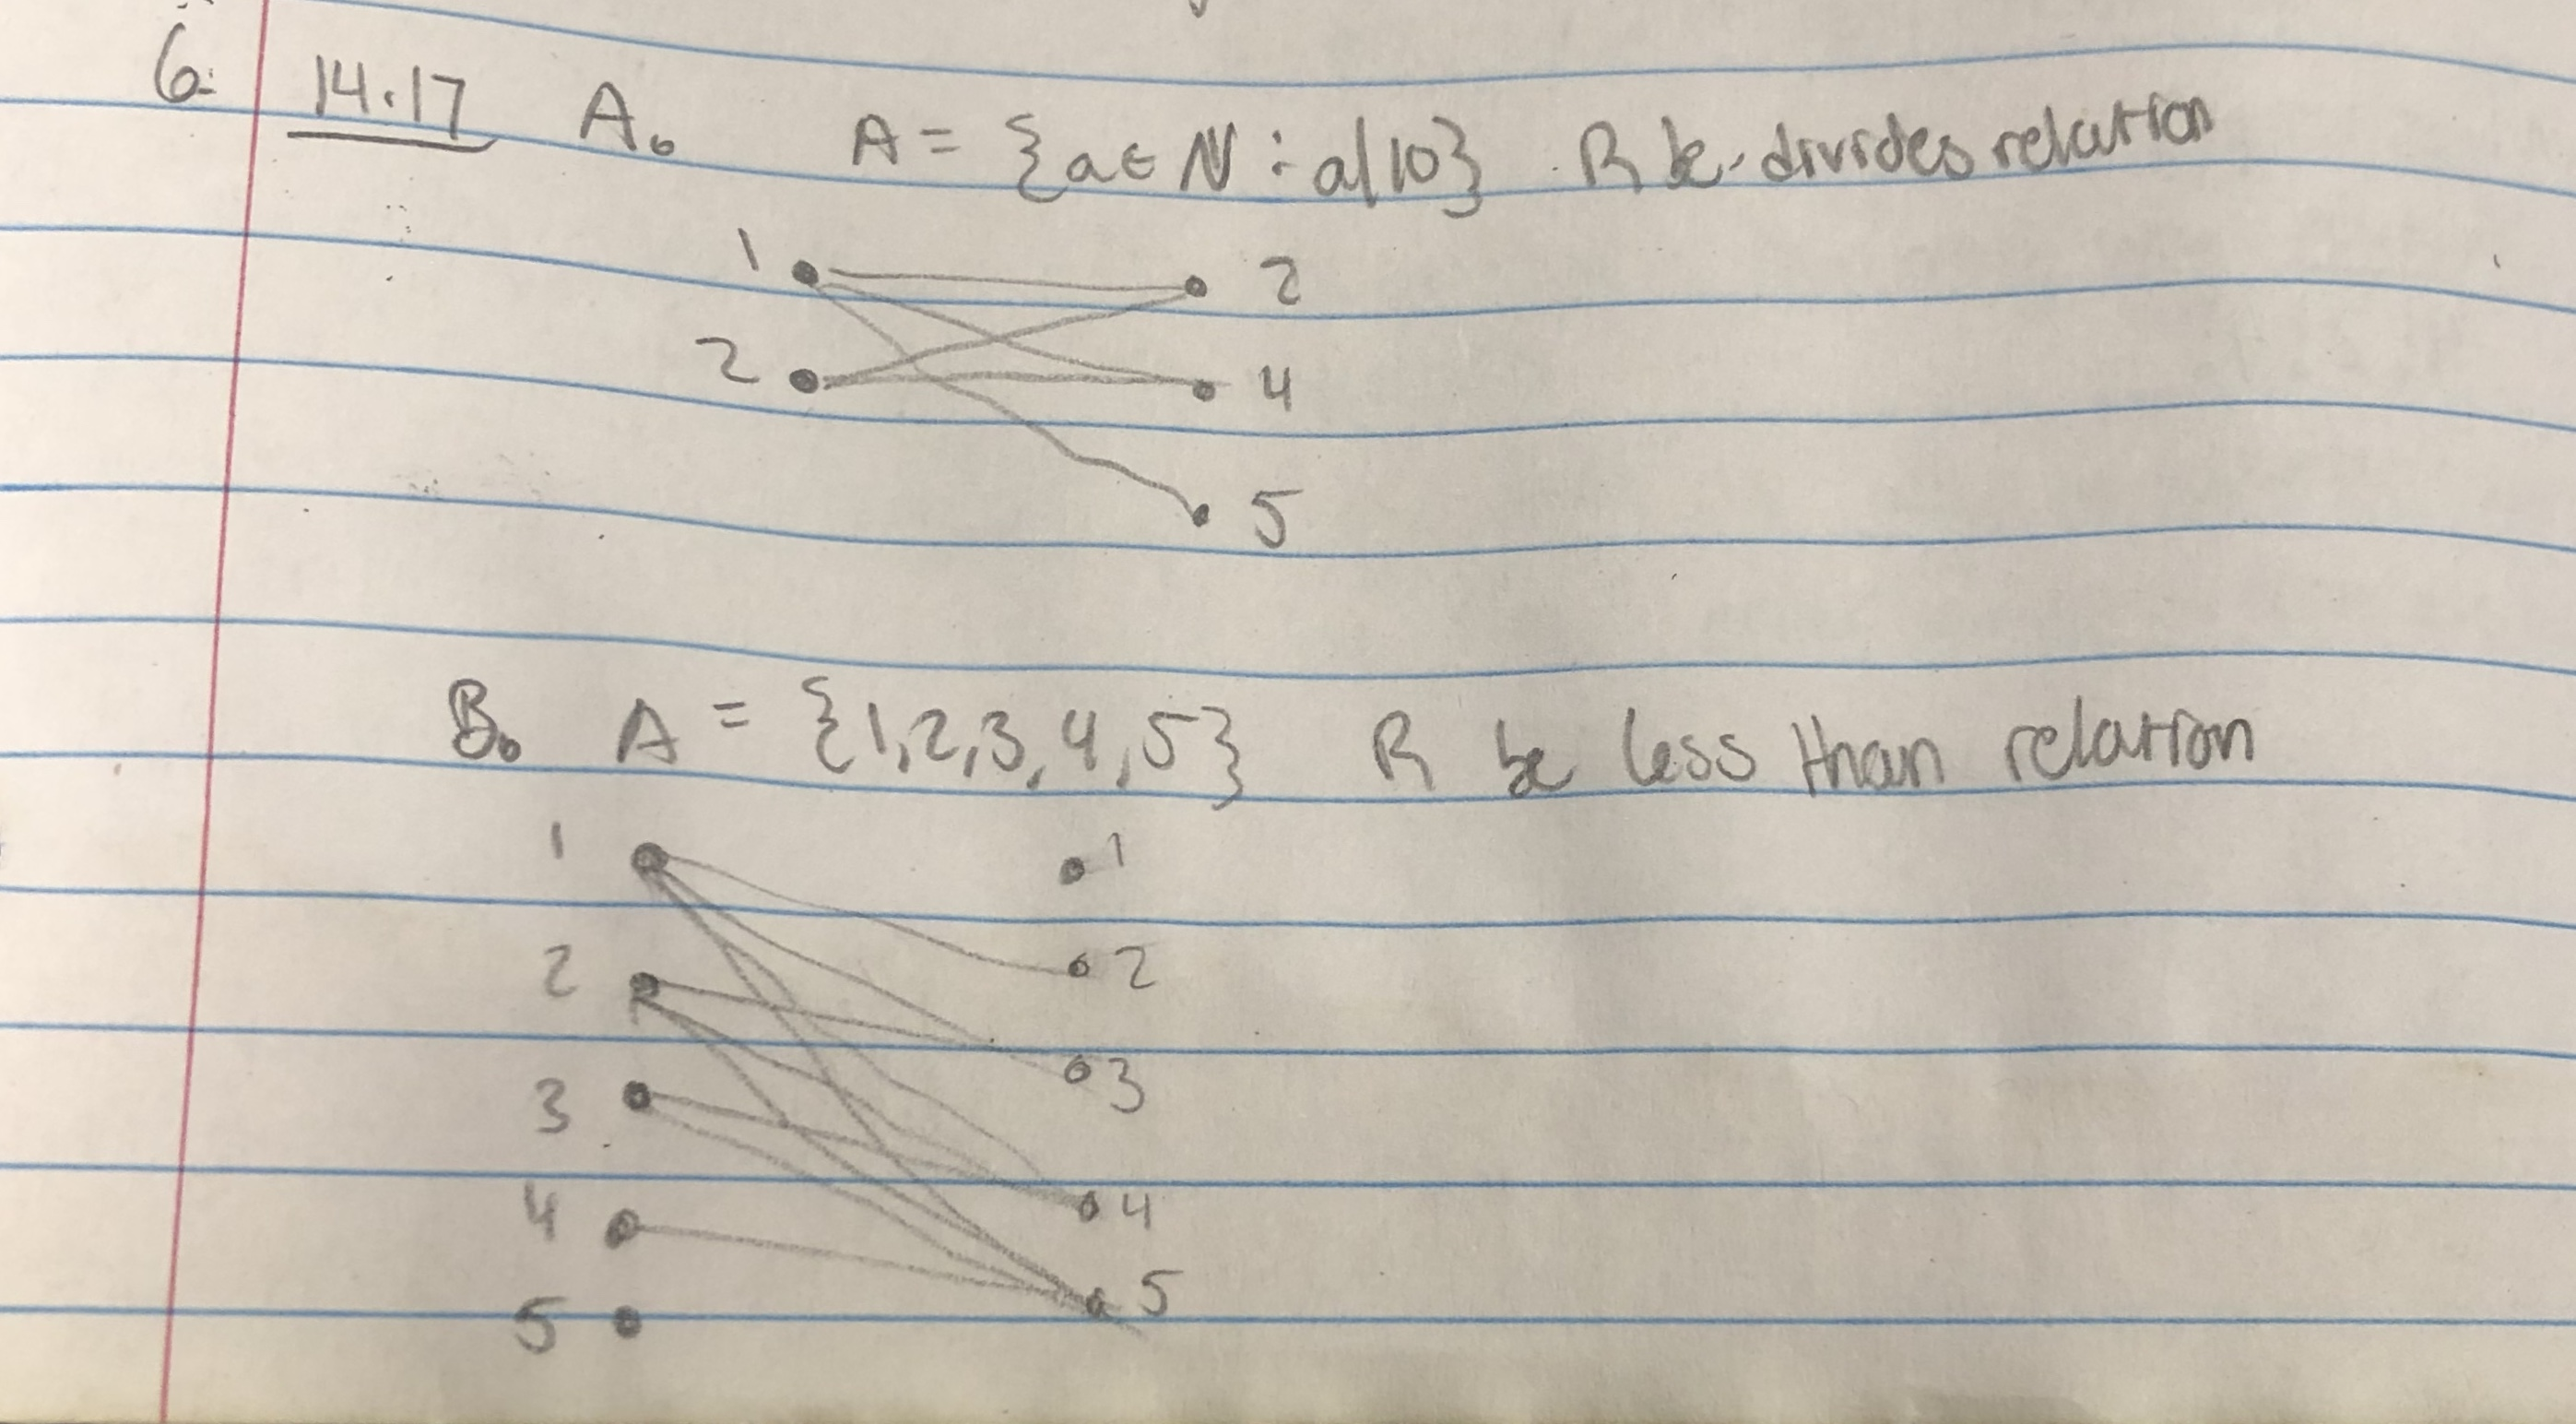
\includegraphics[width = 7in, height = 3in]{HW5_1.jpg} %your jpg file goes between the curly brackets.  To size it, play around with the syntax between the square brackets.  
\]
\\
\[
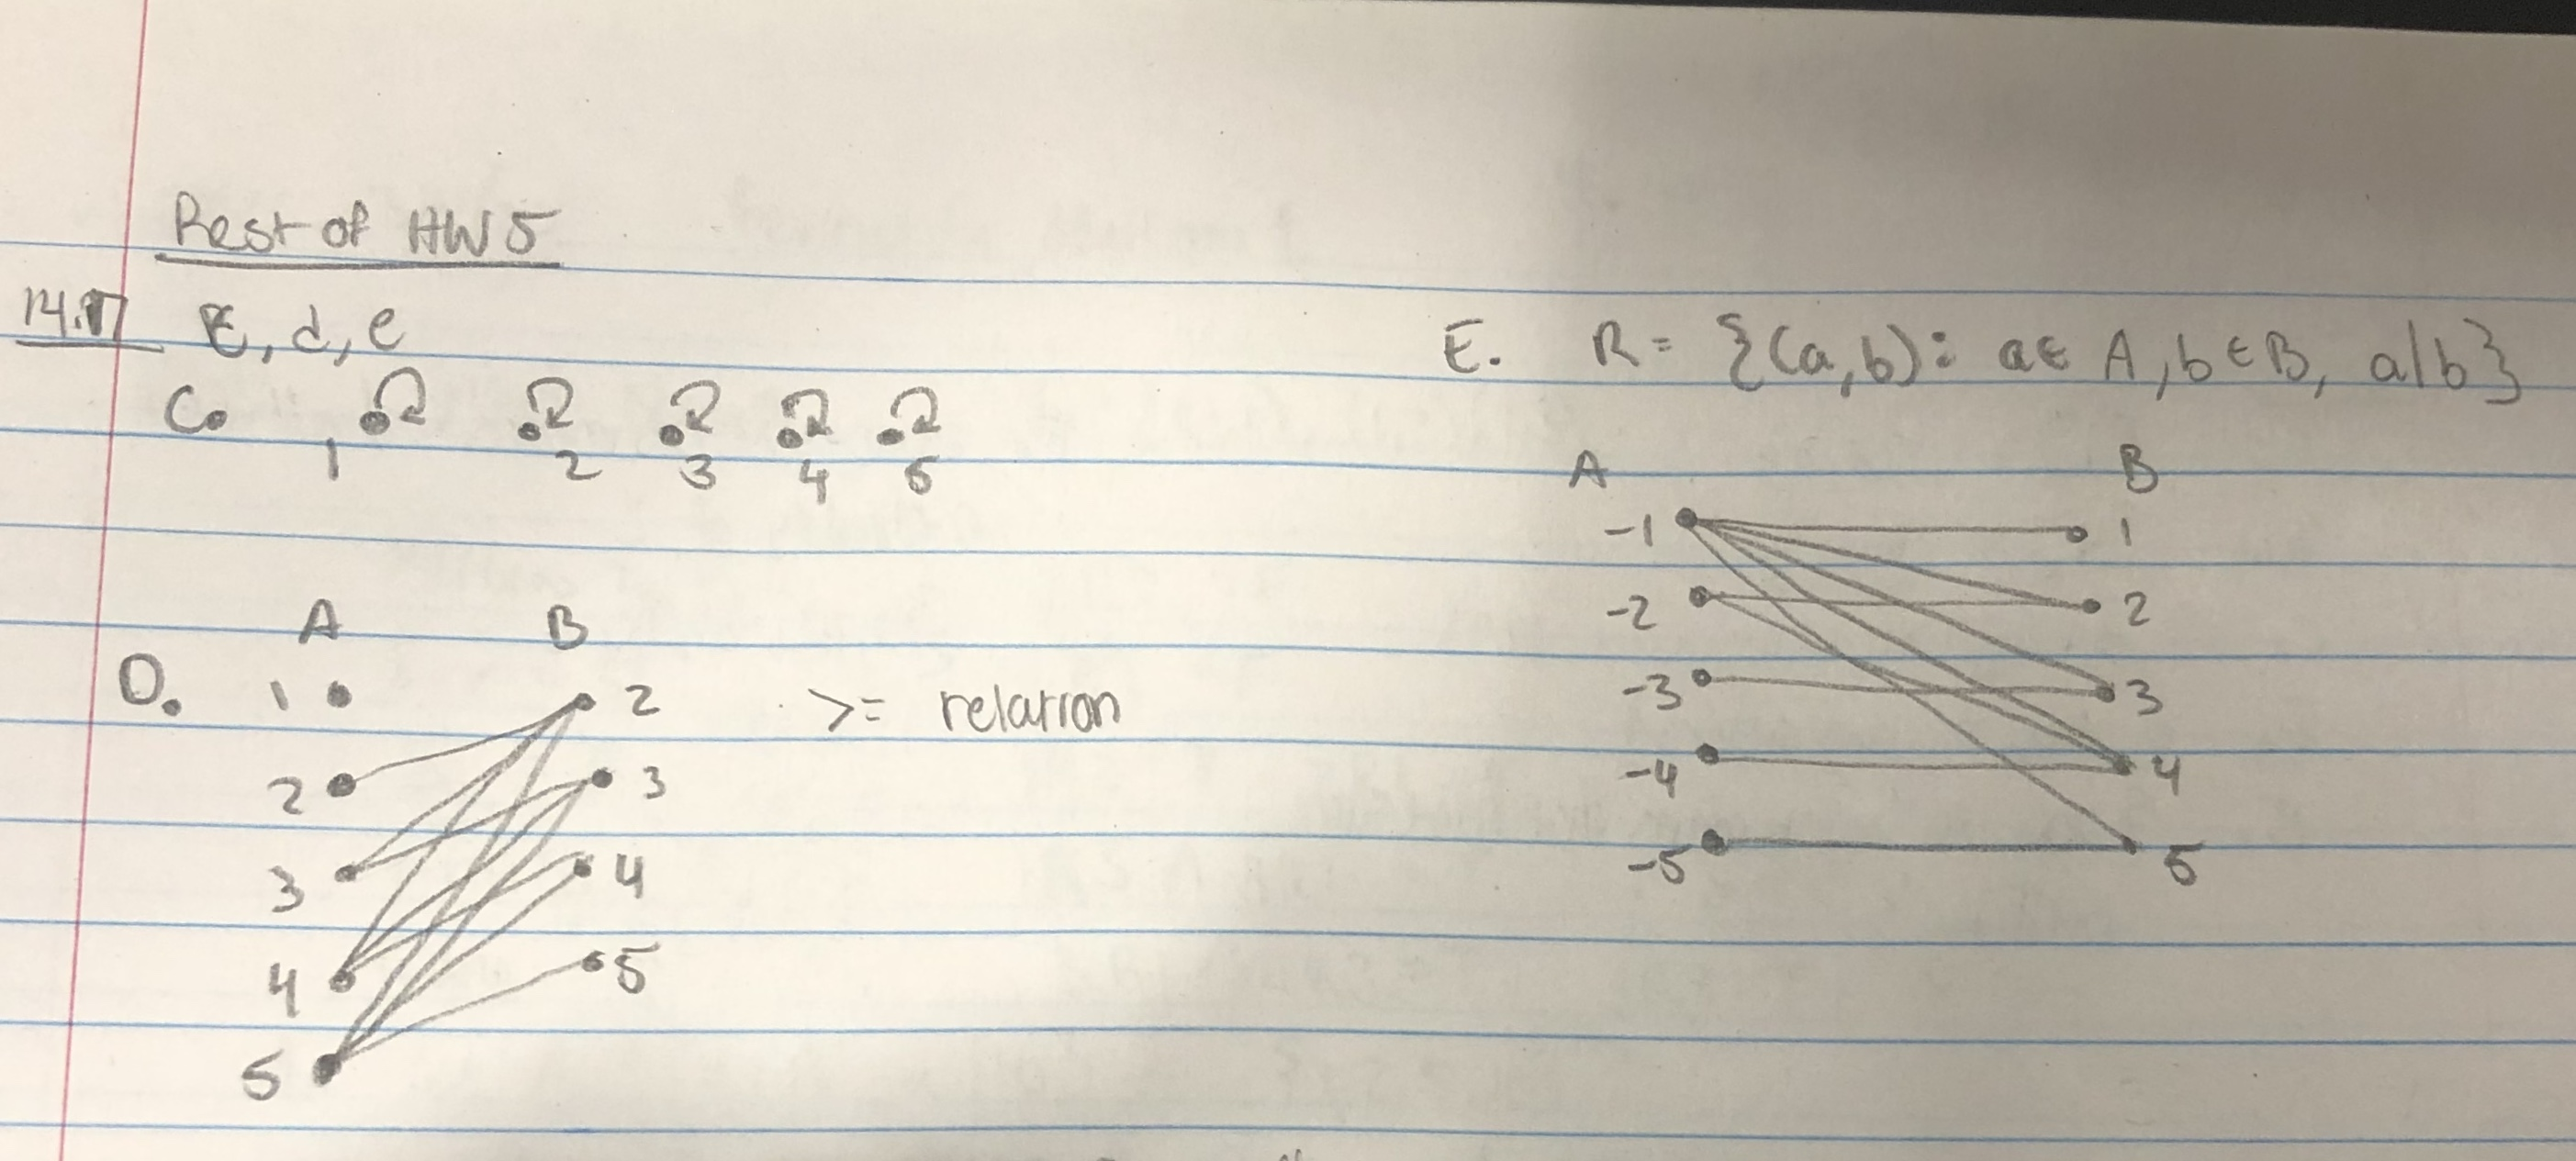
\includegraphics[width = 7in, height = 3in]{HW5_2.jpg} %your jpg file goes between the curly brackets.  To size it, play around with the syntax between the square brackets.  
\]


\item  (21 points) 15.3 \\
\textbf{Solution} \\ 
 A) TRUE  \\
 B) FALSE  \\ 
 C) FALSE  \\
 D) FALSE \\ 
 E) TRUE \\
 F) FALSE \\ 
 G) TRUE \\ 



\item (18 points) 15.7
\textbf{Solution}  \\
 15.7(a) $[1]= \{1,2\}$\\
15.7(b) $[4]=\{4\}$\\
15.7(c) $[123]=\{120,121,122,124,125,126,127,128,129\}$\\
15.7(d) $[you]=\{you,your\ siblings\}$\\
15.7(e) $[you]=\{you,people\ born\ on\ the\ same\ day\ as\ you\}$\\
15.7(f) $[\{1,3\}]=\{\{1,2\},\{1,3\},\{1,4\},\{1,5\},\{2,3\},\{2,4\},\{2,5\},\{3,4\},\{3,5\},\{4,5\}\}$\\


\item (12 points) 15.8 \\
A: There are 10 distinct equivalence Classes \\
B: 365 equivalence classes \\
C: 8 equivalence classes \\
D: 50 equivalence classes \\

\item (3 points) 15.9

$[1]=\{x \in \mathbb{Z}: x \equiv 1\ (mod\ 2)\}$\\
this means for all integers the form will be 
\[
\begin{aligned}
2\mid (x-1)&= \\
x-1&=2k\\
x&=2k+1\\
\end{aligned}
\]
So it's the set of odd numbers .\\

$[3]=\{x \in \mathbb{Z}: x \equiv 3\ (mod\ 2)\}$\\
this means for all integers the form will be 
\[
\begin{aligned}
2\mid (x-3)&= \\
x-3&=2k\\
x&=2k+3\\
x&=2k+2+1\\
x&=2(k+1)+1\\
x&=2m+1 \;\;\; \textit{where }m=k+1
\end{aligned}
\]
They both have the set of odd numbers as their answer. $\square$


\end{enumerate}




\end{document}